\documentclass[11pt,a4paper]{ivoa}
\input tthdefs

\usepackage{array}
\usepackage{tabulary}  % for nicer tables
\usepackage{calc}
\setlength\extrarowheight{2pt}

\newcolumntype{L}{>{\centering\arraybackslash}m{3cm}}

\title{Vodml-instance-vot}

% see ivoatexDoc for what group names to use here
\ivoagroup{DM}

\newcommand{\TODO}[1]{%
    \noindent%
    \colorbox{todocolor}{%
            \parbox{0.85\linewidth}{\sffamily \textbf{TODO:}\\
            #1}
    }%
    \vspace{2pt}

}

\newcommand{\note}[1]{%
    \noindent%
    \textcolor{darkgrey}{{\sffamily Note:} \emph{#1}}%
}

\newcommand{\comment}[1]{%
    \noindent%
    \textcolor{red}{{\sffamily Comment:} \emph{#1}}%
}

\definecolor{todocolor}{rgb}{1,1,0.8}
\definecolor{darkred}{rgb}{0.6,0,0}
\definecolor{rose}{rgb}{1.0,0.88,0.88}
\definecolor{darkgrey}{rgb}{0.35,0.35,0.35}
\definecolor{gray}{rgb}{0.4,0.4,0.4}
\definecolor{darkblue}{rgb}{0.0,0.0,0.6}
\definecolor{maroon}{rgb}{0.5,0,0}
\definecolor{cyan}{rgb}{0.0,0.6,0.6}

\lstset{
  basicstyle=\ttfamily,
  columns=fullflexible,
  showstringspaces=false,
  commentstyle=\color{gray}\upshape
}

\lstdefinelanguage{XML}
{
  morestring=[b]",
  morestring=[s]{>}{<},
  morecomment=[s]{<?}{?>}, 
  morecomment=[s]{<!--}{-->},
  stringstyle=\color{black},
  identifierstyle=\color{darkblue},
  keywordstyle=\color{maroon},
  morekeywords={ref,utype,dmrole, dmtype, value}% list your attributes here
}

\lstdefinestyle{XML}{
    captionpos=b,
    basicstyle=\small\ttfamily
}
\author{François Bonnarel}
\author{Gilles Landais}
\author{Laurent Michel}
\author{Jesus Salgado}

\editor{Laurent Michel}

% \previousversion[????URL????]{????Concise Document Label????}
\previousversion{This is the first public release}
       

\begin{document}

\begin{abstract}
Vodml-instance-vot proposes a syntax to map VOTable data on any model serialized in VO-DML.
Vodml-instance-vot annotations are grouped in a single XML block located in the VOTable head. The annotation block allows to easily reconstruct the model structure. It designed in a way that the block can be reused on different data sets in order to facilitate the annotation process.
Vodml-instance-vot is enable to join data from different tables
\end{abstract}


\section*{Acknowledgments}
CDS/TDIG/SourceDM contributors

\section*{Conformance-related definitions}

The words ``MUST'', ``SHALL'', ``SHOULD'', ``MAY'', ``RECOMMENDED'', and
``OPTIONAL'' (in upper or lower case) used in this document are to be
interpreted as described in IETF standard RFC2119 \citep{std:RFC2119}.

The \emph{Virtual Observatory (VO)} is a
general term for a collection of federated resources that can be used
to conduct astronomical research, education, and outreach.
The \href{http://www.ivoa.net}{International
Virtual Observatory Alliance (IVOA)} is a global
collaboration of separately funded projects to develop standards and
infrastructure that enable VO applications.


\section{Introduction}
The first purpose of a model is to provide,  for a particular domain, a formal description of the relevant quantities and of the way they are connected together .
This documentary role facilitates the communication between the stack-holders and thus the design of interoperability protocols. 

At data level, interoperability consists in arranging searched data in a way that a client can understand them without taking care of their origin. So that, the same code can process and compare data coming from different sources.  That way to arrange data is given by the model.

This is not done by default with VOtables because VOTables are containers. The VOTable schema cannot say how data are mapped on a given model or whether they match any model at all. This is not an issue for simple protocol responses (ref) because the VOTable structure is defined by the protocol itself but this is however a big issue for VOTables containing native data such as Vizier  or TAP query responses.

The challenge here is to bind native data with a given model in a way that a model aware software can see them as model instances while maintaining the possibility to access them in their original forms.

This is partially done with UTypes which may connect FIELDs or PARAMs with model leaves in the case of simple tree-views of the model. Unfortunately, there is no more unique  way to build and parse UTypes in the context of more complex the models. This occurs when e.g the same class is used in different location of the model or when the model contains loops. It is also not possible to refer data from different tables with  UTypes.

%Fb : "This is just because UTypes have been invented at a period when there was no standard way to formally describe  models." Actually it's more complex than that. As long as the model instances are flat or simple trees (charcaterisation) utypes may work. When you have some loops (like in complex Provenace queries) utypes are not enough to map the structure of instances (corrected LM)

The landscape has dramatically changed in 2016 when VODML (ref) became a recommendation. VODML is a meta-model that gives a standard way to design VO models and to make them machine-readable.
%FB: if we have the reference we don't need "which is a rec since é016" (fixed LM)
In VODML, model leaves are no longer identified by a simple string like UTypes do but by a certain role played in a given location in the model hierarchy.
The consequence is that any annotation mechanism based on VODML must preserve the model hierarchy to save the role played by any components. In this context, it might be easy to re-construct model instances from the annotations. 
%FB: see above the actual difference between utype strategy and vodml lite mapping (fixed LM)
%FB : I don't understand at all following sentence "This is very interesting because a copy that model hierarchy with leaves set with real data is nothing else that a model instance which is exactly what we need to be interoperable." (fixed LM)

The main concept of VODML mapping is to insert on  top of the VOTable an XML block following the model structure and containing references to the actual data.
In such a way that in order to build a model instance, a model-aware client only has to make a copy of that structure and to resolve the references. More generic model-unaware clients can just ignore the mapping block. This approach, has been proposed by (GL and OL). 

We have tested the syntax originally proposed and it turned out that it was not well suited for archival data or for TAP responses where the annotation process must be automated as much as possible (entirely for TAP). 

Vodml-instance-vot is based on the same principles as the original proposal but with a particular attention given to the annotation of archival data by keeping focused on both client needs and easiness of the annotation process.
This requires the syntax to be as simple as possible and as flexible as possible to be usable with a wide range of data sets.
% LM does not undertsand this sentence: We must emphasize that we are actually mapping on the data a representation of a peculiar set of instances of the model and not the general model itself.
With Vodml-instance-vot, the model hierarchy is built upon attributes, tuples and arrays (ATTRIBUTE, INSTANCE and COLLECTIONS). Some other elements have been added to guide the parser (FILTER, TABLE\_ROW\_TEMPLATE ...)

%FB : I don't understand why they are the basic elements (simple values,  tuples and  lists, like JSON) Is that VALUE, ARRAY?COMPOSITION ?  
The connections with the data are setup by XML element attributes, so that the mapping structure just depends on the model but not on the mapped data.
%FB : Actually only "ref" attribute ? (ref, tableref, dm_ref, value)

These ideas were first tested in the framework of the TDIG on VOTABLEs containing time series provided by different missions such as Gaia or ZWICKI. 
Then, the syntax has been refined to be used to validate the Mango model on real data.

\iffalse
 The annotation process 

we though it was woth, has been tested on various data. We reached the conclusion that the annotations was not well suited for archival data.

 

 UTypes have been replaced with short identifiers which role depends on 


This is legacy from a period 
This is why the Utype based data annotation has been withdrawn

This is partially done with GROUPs that allow to gather FIELDs and PARAMs into hierarchical structures. Unfortunately, the model elements, in the current VOTable spec (ref) are identfied by Utypes. There is no standard way to construct UTypes and this to parse them. In other, client software has to manage UType list. IN fact 

If  


This can be achieved at protolol level by having a 1-1 association between protocol and  model. With this approach, used for all VO simple protocols (ref), the query responses have a fixed format to which the data must conform. The VOTable FIELDs and PARAMs are defined by the protocol.


associating one model with
The model can also be used by the data provider to expose data in a view
This scope can be extended if we make the model machine readable.


There is no VO standard specifying how to map real data on a model. 
This shortcoming is a bottleneck for interoperability since there is no clean way to compare the same quantities but from differents datasets. 


The model mapping currently used is based on GROUPs. GROUP is a VOTable feature that allows to gather FIELDs and PARAMs into hierarchical structures. In theory, this could be used to map models. Unfortunately, in VOTables, GROUPS haven been used long time before we a standard  

This is satisfactory in many cases but with some limitations however:\begin{enumerate}
   \item The GROUPs, as they are currently used, do not reflect the complete model structure. The are mostly used to group columns with a loose coupling with the model hierarchy. This prevents the restore complex data structures.
   \item The identification of the GROUP elements is based on Utypes which are not clearly connected with the underlying model. Utypes are actually used to represent simple structures. In the current implementations, the client knows the data structures (e.g. coordinate system) and pick values within the group to fill them..
\end{enumerate}
These limitations were unavoidable while we had no common way to represent  models. It is indeed difficult to imagine a consistant model mapping mechanism if there is no standard serialization schema for those models. The situation changed with the usage of VODML. VODML proposes a robust way to make models machine-readable. With VODML, we can consider a mapping syntax directly derived from the model serialization. There are 2 approaches that might be complementary. 
\begin{enumerate}
   \item The first option is to hide the model complexity by flattenning its representation. This is the way GROUPs do work. This approach has the advantage of being compact but it has some strong limitations such as the impossibility of having different elements playing the same role (e.g. 2 position columns in the same table)
   \item The second option consists in keeping the model structure even if this leads to more complex annotations.
\end{enumerate}


Vodml-instance-vot is based on the second option with a particular concern for the process of archival data annotation. The purpose of the VODML mapping in VOTables is to provide a bridge between the data and the model it refers to. The goal of the mapping processing is to make possible to build instances set with values taken out the data tables. In theory, a perfecly faith mapping should be capable of rendering any model feature. In our opinion this ambitious goal led to a mapping syntax difficult to manage.
We prefer to discard this round-trip requirement and to keep focused on both client needs and easiness of the annotation process.

Our main use case is the annotation  of pre-existing data. This  means the annotation process must succeed whatever the way data are arranged even if they do not contain all quantities requested by the model.  
We consider that we have to provide clients with both a data hierarchy view as simple as possibel and an accurate description of the used coordinate systems. 

For most of the usages (display, plot, match, computation),  complex data hierarchies can be wrapped in 3 basic types, the simple values,  tuples and  lists. Vodml-instance-vot  has been built upon these 3 types with a few others annotations guiding the parser.

These ideas that led to this proposal were first tested in the framework of the TDIG on VOTABLEs containing time series provided by different missions such as Gaia or ZWICKI. Then the syntax has been refined to be used to validate the Mango model on real data.

\fi
%The identification of the GROUP elements is based on Utypes which are not clearly connected with the underlying model. Utypes are actually used to represent simple structures. In the current implementations, the client knows the data structures (e.g. coordinate system) and pick values within the group to fill them..



%The current proposal 



%This standard comes after many discussions in the VO about the syntax to be used to annotate VOTable. 
%The ideas that led to this proposal were first tested in the framework of the TDIG on VOTABLEs containing time series provided by different missions such as Gaia or ZWICKI. Then the syntax has been refined to be used to validate the Mango model on real data.

%The existing mapping based on GROUP works fine with the simplest cases. It has the disadvantage of being based on Utypes which are not clearly connected with the underlying model. Utypes are actually used to represent simple structures. In the current implementations, the client knows the data structures (e.g. coordinate system) and pick values within the group to fill them.

 %For now, mone discover or reconstruct a classe hierarchy from groups either. 
%The purpose of the VODML mapping in VOTables is to provide a bridge between the model it refers to and the data. The mapping processing is meant to deliver a model instance set with values taken out the data table. In theory, a perfecly faith mapping should be capable of rendering any model feature. In our opinion this ambitious goal led to a mapping syntax difficult to manage.
%We prefer to discard this round-trip requirement and to keep focused on the client needs and the easiness of the VOTable annotation process.

%ur main use case is the annotation  of pre-existing data. This  means the annotation process must succeed whatever the way data are arranged even if they do not contain all quantities requested by the model.  We consider that the client just needs to reconstruct the data hierarchy and to get a full description of the used coordinate systems. For most of the usages (display, plot, match, computation),  complex data hierarchies can be wrapped in 3 data types, the simple values, the tuples and the lists. The mango mapping has been built upon these 3 types with a few others annotations guiding the work of the parser.

\lstset{language=XML}

\subsection{Role within the VO Architecture}

\begin{figure}
\centering

% As of ivoatex 1.2, the architecture diagram is generated by ivoatex in
% SVG; copy ivoatex/archdiag-full.xml to archdiag.xml and throw out
% all lines not relevant to your standard.
% Notes don't generally need this.  If you don't copy archdiag.xml,
% you must remove archdiag.svg from FIGURES in the Makefile.

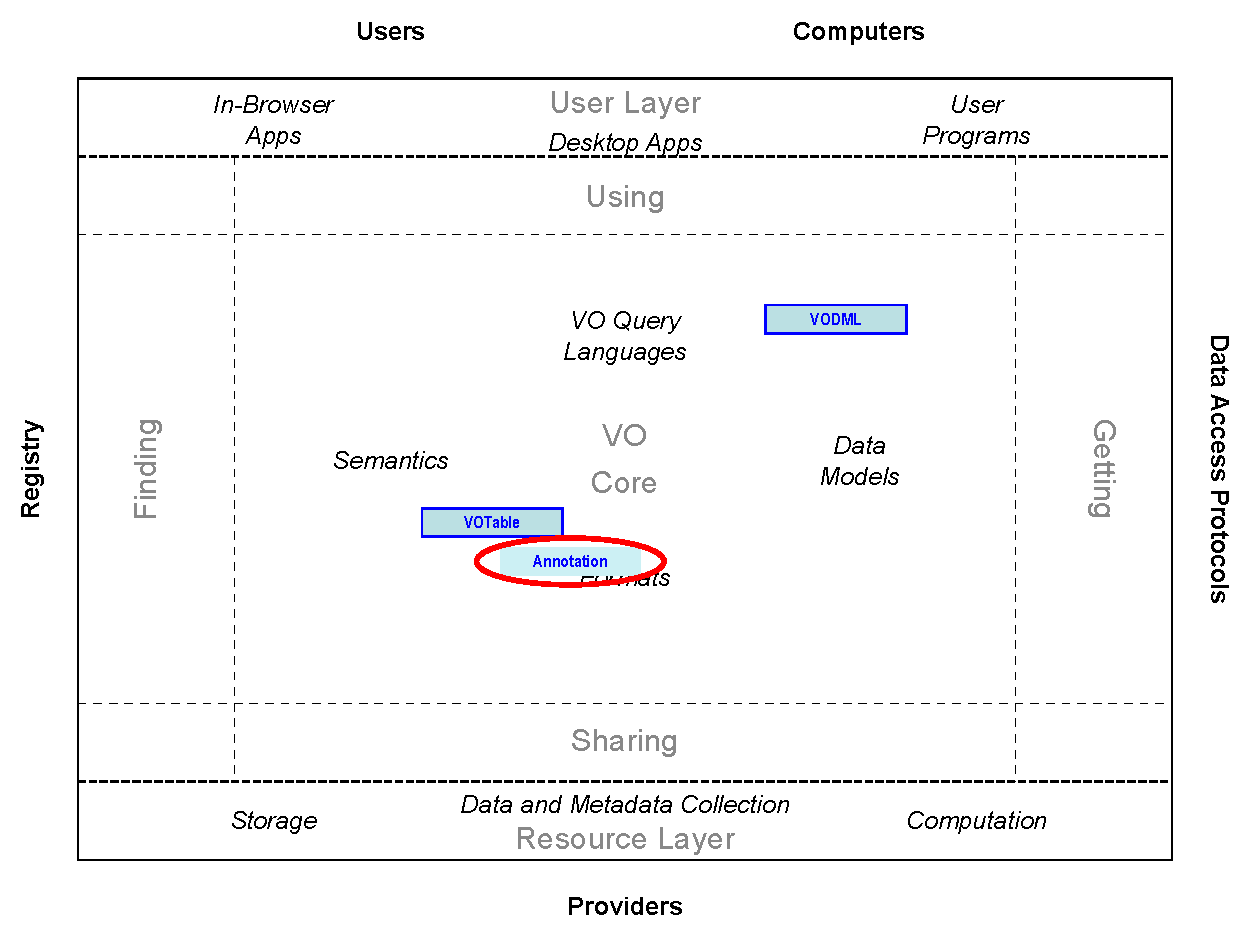
\includegraphics[width=0.9\textwidth]{role_diagram.pdf}
\caption{Architecture diagram for this document}
\label{fig:archdiag}
\end{figure}

Fig.~\ref{fig:archdiag} shows the role this document plays within the
IVOA architecture \citep{note:VOARCH}.

???? and so on, LaTeX as you know and love it. ????

\section{Use Cases and Requirement}

\subsection{Use Cases}

\subsubsection{Client Side}

The mapping is self consistent. The role of the mapping is to give the client all information it needs to reconstruct a datastructure similar to a set of instances of the the model. 
A model-aware client must be able to do this without implementing any code specific to any particular model.  The mapping syntax is independant of the model. The structure of the mapped model is given by the arrangement of the mapping elements, not by the elements themselves

\textbf{Identifying the nature of the content of a VOTable}: A client can get it by a quick look at the annotation block.

\textbf{Measurement discovery}: A client wants to discover whether a VOTable contains some peculiar measurements (position, velocity...). The annotation block allows it to get an answer by a quick parsing of the annotation block.

\textbf{Data set comparison}: A client wants to compare different data set (Xmatch, plot). The annotation provides a homogeneous data representation of these data that allows to put them together in a consistent way. 

\textbf{Data set export}: A client wants to export (e.g. with SAMP) a model instance in a convenient format (e.g. json). The JSON model instance can be buit from the annotation block and exported to a another party.

\subsubsection{Server Side}
The server use cases are to make possible the realization of those of the clients  for a reasonable cost. The annotation process can represent a significant extra work for the curator team that must be limited as much as possible. To do so the mapping syntax is designed to facilitate the use of templates and components.

3 server types that could annotate data have been identified:
\begin{enumerate}
   \item Mission data provider: the data annotation can be set once forever for each data product at the design phase.
   \item Archival data provider: The data annotation must be done for each archived datat set. The curator has a little control, on the data format and he/she has to do his best to match data with the model(s) 
   \item  TAP data provider: In case of TAP services, the annotation process is in charge of the TAP server that must dynamically  match the queried data with the model quantities for each specific query.
\end{enumerate}

The goal of this version of the specification is to support requirements 1) and 2) with a special attention to make 2) easier. Support of requirement 3) is still an experimental feature at the time this specification is written.


\subsection{Requirements}

\begin{itemize}
\item Shy Annotations: The data mapping must not affect the operation of existing clients.

\item Faithful Annotations: The structure of the annotation must be faithful to any VODML compliant model. 


\item Different Usage Levels 
\begin{itemize}
   \item The data mapping must be easily ignored by the client.
   \item The data mapping must allow clients to easily detect the model on which data are mapped.
   \item The data mapping must allow clients to easily get the general metadata (e.g. coordinate systems).
   \item The data mapping must allow clients to get full model instances for each table row.
\end{itemize}

\item Easy to Build 
\begin{itemize}
   \item The mapping structure must be independent of the data structure.
   \item The mapping syntax should make easy the building of both mapping components and templates.
\end{itemize}

\item Complex Data Mapping 
\begin{itemize}
   \item The mapping syntax must support to retrieve data spread over several tables.
   \item The mapping syntax must be able to filter data rows which are part of a specific instance.
   \item The mapping syntax must be able to group data rows in an set of instances.
\end{itemize}
\end{itemize}


\section{Syntax}


The syntax specified in this standard gives rules to build consistent annotations for any model. However, it do not prevent to do foolish things, in the same way that a programming language grammar does not protect people against writing irrelevant software.
In the follwoing examples, attribute values do not refer toi any particular model or VOTable. They have been to help reader to figure out their meanings.

\subsection{Mapping Block Structure}

\textit{The rules below must be updated accordingly to the XML schema .. in progress....}

The mapping block is outside of the data tables. Its scope is the whole VOTable. Its stucture is given below.

\begin{lstlisting}[caption={INSTANCE bloc example},style=XML]
 <VODML>
    <MODELS>   ...  </MODELS>
    <GLOBALS>   ...  </GLOBALS>

    <TEMPLATES tableref=...>  ... </TEMPLATES tableref=...>
    <TEMPLATES tableref=...> ...  </TEMPLATES tableref=...>
    ...
 </VODML>
\end{lstlisting}

The mapping construction rules are the same whatever the model or the data layout are.

\begin{itemize}
    \item The mapping is located in a \texttt{<VODML>} block, child of \texttt{<VOTABLE>}.
    \item The mapping elements reflect the model structure.
    \item The \texttt{<VODML>} block starts with a list of implemented models.
    \item There is one \texttt{<TEMPLATES>} per mapped \texttt{<TABLE>}.
    \item There is one \texttt{<GLOBALS>} block containing data shared by the whole mapping.
\end{itemize}

%%%%%%%%%%%%%%%%%%%%%%%%%%%%%%%%%%%%%
%
% MODELS
%
\subsection{MODELS}

The  \texttt{MODELS}  blocks contains the list of the models mapped in the block. It can be left empty.


\begin{itemize}
    \item Models referenced in \texttt{MODELS} are not necessary VO standards, but they must be accessible by a VODML URI.
    \item It is to be noted that the mapping syntax allows to reconstruct the model structure without parsing any VODML model serialization.
\end{itemize}

\begin{lstlisting}[caption={GLOBALS block example},style=XML]
<MODELS>
    <MODEL>
        <NAME>ivoa</NAME>
        <URL>http://www.ivoa.net/xml/VODML/IVOA-v1.vo-dml.xml
        </URL>
    </MODEL>
    <MODEL>
        <NAME>coords</NAME>
        <URL>http://www.ivoa.net/xml/STC_coords-v1.0.vo-dml.xml
    </URL>
    </MODEL>
    <MODEL>
        <NAME>meas</NAME>
        <URL>http://www.ivoa.net/xml/STC_meas-v1.0.vo-dml.xml
        </URL>
    </MODEL>
</MODELS>
\end{lstlisting}

 \texttt{MODELS},  {MODEL},  {NAME} and {URL}  have no attributes. 
 

%%%%%%%%%%%%%%%%%%%%%%%%%%%%%%%%%%%%%
%
% GLOBALS
%
\subsection{GLOBALS}
 Contains  \texttt{INSTANCE}s  that can be used everywhere in the \texttt{VODML}.
\begin{itemize}
    \item \texttt{INSTANCE}s children of \texttt{GLOBALS} should have an  \texttt{@ID} attribute so that they can be referenced from other instances.
    \item The role of the \texttt{GLOBALS}s children (\texttt{INSTANCE} by construction) must be ignored although being mandatory.
    \item References within \texttt{GLOBALS}s  sub-elements to VOTable data (\texttt{FIELD} ot \texttt{PARAM}) must be searched in all tables. 
            They must be resolved by the first occurence matching the reference found.
    \item \texttt{GLOBALS} has no attributes. 
\end{itemize}

\begin{lstlisting}[caption={GLOBALS block example},style=XML]
  <GLOBALS>
    <INSTANCE ID="SpaceCoordFrame" dmrole="">
      <INSTANCE dmrole="coords:SpaceFrame.refPosition" 
                 dmtype="coords:StdRefLocation">
          <ATTRIBUTE dmrole="coords:StdRefLocation.position" 
                      dmtype="ivoa:string" value="NoSet"/>
      </INSTANCE>
      <ATTRIBUTE dmrole="coords:SpaceFrame.spaceRefFrame" 
                  dmtype="ivoa:string" value="ICRS"/>
      <ATTRIBUTE dmrole="coords:SpaceFrame.equinox" 
                  dmtype="coords:Epoch"   value="NoSet"/>
    </INSTANCE>
 </GLOBALS>
\end{lstlisting}




\begin{table}[hbtp]
\small
\centering
\begin{tabulary}{\linewidth}{|c|J|}       
       \hline 
           \textbf{Child} &  
           \textbf{Role}\\
       \hline         \hline  
            \texttt{INSTANCE}    &  
            Model instances with a scope covering the whole VOTable . \\       
       \hline 
     \end{tabulary}
     \caption{Allowed  \texttt{GLOBALS} children} 
     \label{tbl:globals-children}
 \end{table}


%%%%%%%%%%%%%%%%%%%%%%%%%%%%%%%%%%%%%
%
% TEMPLATES
%
\subsection{TEMPLATES}

\texttt{TEMPLATE} blocks contain the mapping statements of the data contained in one \texttt{TABLE} .

\begin{itemize}
    \item There is one \texttt{TEMPLATE} block for each mapped \texttt{TABLE}  in the VOTAble    
    \item A \texttt{TABLE} cannot be referenced by more than one \texttt{TEMPLATE}.
    \item  There is \texttt{TEMPLATE} reference ( @\texttt{tableref} ) must be first resolved against the \texttt{TABLE} identifier (  @\texttt{ID} ).
\end{itemize}

\begin{lstlisting}[caption={GLOBALS block example},style=XML]
<TEMPLATES tableref="OtherResults">
    <COLLECTION dmrole="test:detections">
        <TABLE_ROW_TEMPLATE>
            <INSTANCE dmrole="test:detection" dmtype="test:Detection">
               <ATTRIBUTE dmrole="test:detection.num" dmtype="ivoa:real"
                           ref="_num_148" />
               <ATTRIBUTE dmrole="test:detection.id" dmtype="ivoa:real"
                           ref="_foreign" />
           </INSTANCE>
        </TABLE_ROW_TEMPLATE>
    </COLLECTION>
</TEMPLATES>
\end{lstlisting}


\begin{table}[hbtp]
\small
\centering
\begin{tabulary}{\linewidth}{|c|J|}       
       \hline 
           \textbf{Child} &  
           \textbf{Role}\\
       \hline         \hline  
           \texttt{INSTANCE}    & 
           The table data are mapped on these instances.  \\              
       \hline  
            \texttt{TABLE\_ROW\_TEMPLATE}    &  
            There is one instance per table row. 
             \newline The structure of those instance is given by the TABLE\_ROW\_TEMPLATE children \\              
       \hline  
             \texttt{COLLECTION}    &  
             The table data are mapped on an instance list \\       
       \hline 
     \end{tabulary}
     \caption{Allowed  \texttt{TEMPLATES} children} 
     \label{tbl:templ-children}
 \end{table}


\begin{table}[hbtp]
\small
\centering
\begin{tabulary}{\linewidth}{|c|J|}       
       \hline 
            \textbf{Attribute} & 
            \textbf {Role}\\
       \hline         \hline  
            @tableref  & 
            The @ID or the @name of the mapped table  \\
       \hline 
     \end{tabulary}
     \caption{\texttt{TEMPLATES} attributes} 
     \label{tbl:templ-att}
 \end{table}

\begin{table}[hbtp]
\small
\centering
\begin{tabulary}{\linewidth}{|c|c|c|c|J|}
    \hline 
        \textbf{@tableref} &
        \textbf{Pattern}\\
    \hline      \hline  
        MAND &   
        Always mandatory\\
   \hline 
\end{tabulary}
     \caption{Valid attribute patterns for  \texttt{TEMPLATES}} 
     \label{tbl:templ-pattern}
 \end{table}

%%%%%%%%%%%%%%%%%%%%%%%%%%%%%%%%%%%%%
%
% INSTANCE
%
\subsection{INSTANCE}

Mapping for either object types or a datatype instances.


\begin{lstlisting}[caption={INSTANCE block example},style=XML]
<INSTANCE dmrole="ds:Dataset.dataID" dmtype="ds:DataID" ID="_ds_">
    <ATTRIBUTE dmrole="ds:DataID.title" value="Gaia TS Mapping Test" />
    <ATTRIBUTE dmrole="ds:DataID.datasetID" value="ivoa://gaia/ts/12345" />
    <ATTRIBUTE dmrole="ds:DataID.creatorDID" value="ivoa://esa/gaia/" />
    <ATTRIBUTE dmrole="ds:DataID.version" value="0.0" />
    <ATTRIBUTE dmrole="ds:DataID.date" value="2018:11:11" />
    <ATTRIBUTE dmrole="ds:DataID.creationType" value="LiteMappingTest" />
    <INSTANCE dmrole="ds:DataID.creator" dmtype="ds:Creator">
        <INSTANCE dmrole="ds:Role.party" dmtype="ds:party.Individual">
            <ATTRIBUTE dmrole="ds:Party.name" value="VODML-Team" />
       </INSTANCE>
    </INSTANCE>
</INSTANCE>
\end{lstlisting}


\begin{table}[hbtp]
\small
\centering
\begin{tabulary}{\linewidth}{|c|J|}       
       \hline 
           \textbf{Child} &  
           \textbf{Role} \\
       \hline         \hline  
           \texttt{INSTANCE}    & 
           Another embedded instance . \\       
       \hline  
           \texttt{ATTRIBUTE}    & 
           Primitive attribute . \\       
       \hline  
            \texttt{COLLECTION}    & 
           Set of items\\      
       \hline 
     \end{tabulary}
     \caption{Supported  \texttt{INSTANCE} children} 
     \label{tbl:inst-chilrdren}
\end{table}

\begin{table}[hbtp]
\small
\centering
\begin{tabulary}{\linewidth}{|c|J|}       
       \hline 
            \textbf{Attribute} &  
            \textbf{Role}\\
       \hline  
            @dmrole    & 
            VODML role of the instance.  \\
       \hline  
            @dmtype & 
            VODML type of the instance.  \newline Must never be empty \\
       \hline  
            @dmref  & 
            Reference to another instance in the mapping block. 
            \newline  Must never be empty\\          
       \hline  
            @ID  & 
            Unique identifier of the instance. 
            \newline  Must never be empty\\
       \hline 
     \end{tabulary}
     \caption{\texttt{INSTANCE} attributes} 
     \label{tbl:inst-att}
 \end{table}

\begin{table}[hbtp]
\small
\centering
\begin{tabulary}{\linewidth}{|c|c|c|c|J|}
    \hline 
        \textbf{@dmrole} & 
        \textbf{@dmref} &  
        \textbf{@dmtype} &  
        \textbf{@ID} &  
        \textbf{Pattern}\\
    \hline      \hline  
        MAND &   
       & 
       MAND & 
       OPT & 
       Instance of a certain type playing a certain role. 
         \newline The role may be left empty  for child instances of 
          \texttt{GLOBALS} \\
    \hline  
       MAND  & 
       MAND  &  
       &  
       & 
       Reference to another instance. 
        \newline  No allowed children in this case.  \\

\hline 
\end{tabulary}
     \caption{Valid attribute patterns for  \texttt{INSTANCE}} 
     \label{tbl:inst-pattern}
 \end{table}

%%%%%%%%%%%%%%%%%%%%%%%%%%%%%%%%%%%%%
%
% ATTRIBUTE
%
\subsection{ATTRIBUTE}

Mapping statement for primitive attributes.

\begin{itemize}
    \item \texttt{ATTRIBUTE}s  are the model leaves that point onto real data or are set with literals
    \item \texttt{ATTRIBUTE}s have no children.
\end{itemize}

\begin{lstlisting}[caption={ATTRIBUTE examples},style=XML]
<INSTANCE dmrole="model:value.example" dmtype="model:value.Example">
    <ATTRIBUTE dmrole="model:preset.value" value="Preset Value" />    
    <ATTRIBUTE dmrole="model:ref.value" ref="fieldID" />    
    <ATTRIBUTE dmrole="model:refofpreset.value" 
                value="Preset Value" ref="fieldID" />
</INSTANCE>
\end{lstlisting}


\begin{table}[hbtp]
\small
\centering
\begin{tabulary}{\linewidth}{|c|J|}
       \hline 
          \textbf{Attribute} & 
          \textbf{Role}\\
       \hline         \hline  
          @dmrole    & 
           VODML role of the instance attribute.\\       
       \hline 
          @dmtype    & 
          VODML type of the instance attribute.\\
       \hline  
          @value   &
          Literal value of the instance attribute. 
                     \newline If  \texttt{ATTRIBUTE} has also a \texttt{@ref}, \texttt{@ref} MUST be resolved first.
                     \texttt{ATTRIBUTE}  MUST be taken when \texttt{@ref} cannot be resolved \\
        \hline
           @ref & 
            Reference of the data element (\texttt{FIELD} or \texttt{PARAM}).  
                    \newline MUST refer to an element of the \texttt{TABLE}  referenced by the current     
                    \texttt{TEMPLATE}                    
                    \newline The client MUST first look for a \texttt{FIELD} matching \texttt{@ref}. 
                    \newline In case of failure, it MUST look for a \texttt{PARAM}
                    \\
       \hline 
     \end{tabulary}
     \caption{\texttt{ATTRIBUTE} attributes} 
     \label{tbl:att-att}
 \end{table}

\begin{table}[hbtp]
\small
\centering
\begin{tabulary}{1.0\linewidth}{|c|c|c|c|J|}

    \hline    
          \textbf{@dmrole}  &  
          \textbf{@dmtype} &  
          \textbf{@ref} &  
          \textbf{@value} &  
          \textbf{Pattern}\\
    \hline   \hline 
          MAND & 
          MAND &  
          MAND &  
          OPT & 
          The instance attribute must take the value pointed by \texttt{@ref}. 
           \newline If the reference cannot be resolved, the attribute takes the value of \texttt{@val} if present.\newline  It is considered as not set otherwise.   \\
     \hline  
          MAND & 
          MAND &   
          &  
          MAND & 
          The attribute takes the value of \texttt{@val}.   \\
     \hline 
  \end{tabulary}
  \caption{Valid attribute patterns for  \texttt{ATTRIBUTE}} 
  \label{tbl:att-pattern}
 \end{table}



%%%%%%%%%%%%%%%%%%%%%%%%%%%%%%%%%%%%%
%
% COLLECTION
%
\subsection{COLLECTION}
Mapping statement fort sets of instances or collections.

\begin{itemize}
    \item A \texttt{COLLECTION} can contain a fixed set of instances or collections, each one being mapped individually.  
    \item A \texttt{COLLECTION} can contain an unbounded set of instances, one per selected table row. 
            In this case, all items have tyhe same mapping. They can come from the local table or from a joint table.
 \end{itemize}


\begin{lstlisting}[caption={COLLECTION example},style=XML]
<TEMPLATES tableref="Results">
    <COLLECTION dmrole="meas:Measure.errors" size="2">
         <INSTANCE dmref="globald=s_stat_error" />         
         <INSTANCE dmref="globald=s_sys_error" />
    </COLLECTION>
</TEMPLATES>
\end{lstlisting}

\begin{table}[hbtp]
\small
\centering
\begin{tabulary}{\linewidth}{|L|J|}
       \hline 
           \textbf{Child} &
           \textbf{Role}\\
       \hline  
           \texttt{INSTANCE}    & 
           Collection item. A collection can contain multiple instances \\              
       \hline  
           \texttt{COLLECTION}    & 
          Collection item. A collection can contain multiple instances \\       
       \hline  
           \texttt{TABLE\_ROW\_TEMPLATE}    & 
          The collection is populated with with one instance per row of the current table. This element must be only child. \\       
       \hline  
          \texttt{JOIN}    & 
         The collection is populated with data read in another table. The primary join key must be one of the host instance attributes.This element must be only child. \\      
       \hline 
\end{tabulary}
\caption{Supported  \texttt{COLLECTION} children} 
\label{tbl:coll-children}
\end{table}

\begin{table}[hbtp]
\small
\centering
\begin{tabulary}{\linewidth}{|L|J|}
       \hline 
           \textbf{Attribute} & 
           \textbf{Role}\\
       \hline  
          @dmrole    & 
           VODML role of the collection.\\       
       \hline  
          @size    & 
          Collection size.\\       
       \hline 
 \end{tabulary}
 \caption{Supported attributes for  \texttt{COLLECTION}} 
 \label{tbl:att-att}
 \end{table}


\begin{table}[hbtp]
\small
\centering
\begin{tabulary}{\linewidth}{|L|L|J|}
    \hline 
        @dmrole   & 
        @size   &  
        Role\\
    \hline  
       MAND & 
       OPT & 
       Role played by the collection (VODML relation name usually). Cannot be empty \\    
    \hline 
  \end{tabulary}
  \caption{Valid attribute patterns for  \texttt{COLLECTION}} 
  \label{tbl:coll-pattern}
 \end{table}

%%%%%%%%%%%%%%%%%%%%%%%%%%%%%%%%%%%%%
%
% TABLE_ROW_TEMPLATE
%
\subsection{TABLE\_ROW\_TEMPLATE}
This element indicates that one element must be added to the host COLLECTION for each table row.

\begin{itemize}
    \item The mapping if the row data is given by the child INSTANCE
    \item We assume that we have one INSTANCE per row. 
             This makes senses since a collection element cannot be made with more than one instance
\end{itemize}

\begin{lstlisting}[caption={TABLE\_ROW\_TEMPLATE examples},style=XML]
<TEMPLATES tableref="OtherResults">
    <COLLECTION dmrole="test:detections">
        <TABLE_ROW_TEMPLATE>
            <INSTANCE dmtype="test:Detection">
                <ATTRIBUTE dmrole="test:detection.num" dmtype="ivoa:real"
                            ref="_num_148" />
                <ATTRIBUTE dmrole="test:detection.id" dmtype="ivoa:real"
                            ref="_foreign" />
           </INSTANCE>
        </TABLE_ROW_TEMPLATE>
    </COLLECTION>
</TEMPLATES>
\end{lstlisting}

\begin{table}[hbtp]
\small
\centering
\begin{tabulary}{\linewidth}{|L|J|}
       \hline  
          \textbf{Child} &  
          \textbf{Role}\\
       \hline  
          \texttt{INSTANCE}    & 
          Mapping to be applied to table row \\       
       \hline 
     \end{tabulary}
     \caption{Supported  \texttt{TABLE\_ROW\_TEMPLATE} children} 
     \label{trt:row-children}
\end{table}



%%%%%%%%%%%%%%%%%%%%%%%%%%%%%%%%%%%%%
%
% FILTER
%
\subsection{FILTER}

\begin{lstlisting}[caption={FILTER examples},style=XML]
<COLLECTION dmrole="collection_dmrole">
    <TABLE_ROW_TEMPLATE>
        <FILTER ref="column_name" value="matching_column_value"/>
            <INSTANCE dmref="instance_dmref" dmrole="instance_role" />
    </TABLE_ROW_TEMPLATE>
</COLLECTION>
\end{lstlisting}

\begin{table}[hbtp]
\small
\centering
\begin{tabulary}{\linewidth}{|L|J|}
       \hline  
          \textbf{Child} &  
          \textbf{Role}\\
       \hline  
          \texttt{INSTANCE}    & 
          Mapping to be applied to table rows matching the filter \\       
       \hline 
     \end{tabulary}
     \caption{Supported  \texttt{FILTER} children} 
     \label{tbl:filter-children}
\end{table}



%%%%%%%%%%%%%%%%%%%%%%%%%%%%%%%%%%%%%
%
% JOIN
%
\subsection{JOIN}
This element populates the host collection with data taken out from a foreign table and matching the join criteria.

\begin{itemize}
    \item Each matching row of the foreign table is mapped as one instance mapped by the child INSTANCE.
    \item Self-joins  on the local table are allowed.
    \item The join criteria is based on the equality of the column values. 
             The mapping does not specify the way to deal with data types.
\end{itemize}

\begin{lstlisting}[caption={JOIN example},style=XML]
<TABLE_ROW_TEMPLATE>
    <INSTANCE dmrole="primary:point" dmtype="Point">
        <ATTRIBUTE dmrole="test:detection.num" dmtype="ivoa:real"
                    ref="_poserr_148" />
        <COLLECTION dmrole="test.detections">
            <JOIN tableref="OtherResults" primary="_poserr_148"
                   foreign="_foreign">
                <INSTANCE dmrole="test:detection"  dmtype="test:Detection">
                    <ATTRIBUTE dmrole="test:detection.num" 
                                dmtype="ivoa:real"  ref="_num_148" />
                   <ATTRIBUTE dmrole="test:detection.id" 
                                dmtype="ivoa:real"  ref="_foreign" />
                </INSTANCE>
            </JOIN>
        </COLLECTION>
    </INSTANCE>
</TABLE_ROW_TEMPLATE>
\end{lstlisting}


\begin{table}[hbtp]
\small
\centering
\begin{tabulary}{\linewidth}{|L|J|}
\hline
    \textbf{Child} &
    \textbf{Role} \\
\hline
     \texttt{INSTANCE}    &
     Mapping to be applied to the matching rows.  \\       
\hline
\end{tabulary}
     \caption{Supported  \texttt{JOIN} children} 
     \label{tbl:join-children}
\end{table}

\begin{table}[!htbp]
\small
\centering
\begin{tabulary}{\linewidth}{|L|J|}
       \hline
           \textbf{Attribute} &  
           \textbf{Role} \\
       \hline  
           \texttt{@primary}    & 
           Column name of the primary table used  by the join \\       
       \hline  
           \texttt{@foreign}    & 
           Column name of the foreign table used  by the join \\       
      \hline  
           \texttt{@tableref}    & 
           ID or name of the foreign table \\       
       \hline 
\end{tabulary}
\caption{\texttt{JOIN} attributes} 
\label{tbl:join-att}
\end{table}

\begin{table}[!htbp]
\small
\centering
\begin{tabulary}{\linewidth}{|C|C|C|J|}
       \hline
           \textbf{@primary} &  
           \textbf{@foreign} &                     
           \textbf{@tableref} &          
           \textbf{Role} \\
       \hline  
           MAND    &            
           MAND    &            
           MAND    & 
           All attributes must be set in any case \\       
       \hline 
\end{tabulary}
\caption{Valid \texttt{JOIN} attribute pattern} 
\label{tbl:join-patterns}
\end{table}


%%%%%%%%%%%%%%%%%%%%%%%%%%%%%%%%%%%%%
%
% GROUPBY
%
\subsection{GROUPBY}
This element aggrates grouped data in the host collection =.

\begin{itemize}
    \item Each matching row  is mapped as one instance mapped by the child INSTANCE.
\end{itemize}

In the example below:

\begin{itemize}
    \item The collection with @dmrole=test.lightcurves will be populated with a set of collections
    \item Each of these sub-collections is populated with set of instances mapped by  INSTANCE.
    \item All INSTANCEs are built from rows having all the same values for the column source\_name
\end{itemize}

\begin{lstlisting}[caption={GROUPBY examples},style=XML]
<COLLECTION dmrole="test.lightcurves">
    <GROUPBY ref="source_name">
        <INSTANCE dmref="phit_point_dmref" dmrole="photometric point" />
    </GROUPBY>
</COLLECTION>
\end{lstlisting}

\begin{table}[hbtp]
\small
\centering
\begin{tabulary}{\linewidth}{|L|J|}
\hline
    \textbf{Child} &
    \textbf{Role} \\
\hline
     \texttt{INSTANCE}    &
     Mapping to be applied to the matching rows.  \\       
\hline
\end{tabulary}
     \caption{Supported  \texttt{GROUPBY} children} 
     \label{tbl:group-children}
\end{table}

\begin{table}[!htbp]
\small
\centering
\begin{tabulary}{\linewidth}{|L|J|}
       \hline
           \textbf{Attribute} &  
           \textbf{Role} \\
       \hline  
           \texttt{@ref}    & 
           Identifier of the column used for he grouping \\       
        \hline 
\end{tabulary}
\caption{\texttt{GROUPBY} attributes} 
\label{tbl:group-att}
\end{table}

\begin{table}[!htbp]
\small
\centering
\begin{tabulary}{\linewidth}{|C|J|}
       \hline
           \textbf{@ref} &  
           \textbf{Role} \\
        \hline  
           MAND    &            
           All attributes must be set in any case \\       
       \hline 
\end{tabulary}
\caption{Valid \texttt{GROUPBY} attribute pattern} 
\label{tbl:group-patterns}
\end{table}


%%%%%%%%%%%%%%%%%%%%%%%%%%%%%%%%%%%%%
%
% SHORTCUTS
%
\subsection{Shortcuts}
VODML encourgages people to use the ivoa model for the primitive types. 
Some of these types have a complex structures that associate the unit with the value. 
This is the case for the types derived from ivoa:Quantity (ivoa:RealQuantity and ivoa:IntegerQuantity ).
The XML snipper below show the regular mapping for the realQuantity.

\begin{lstlisting}[caption={ivoa:RealQuantity example},style=XML]
<INSTANCE dmrole="coords:PhysicalCoordinate.cval"
dmtype="ivoa:RealQuantity">
    <ATTRIBUTE dmrole="ivoa:RealQuantity.value" dmtype="ivoa:real"
                     ref="col_id" />
    <ATTRIBUTE dmrole="ivoa:RealQuantity.unit" dmtype="ivoa:Unit"
                     value="m/sec" />
</INSTANCE>
\end{lstlisting}



A this block maps a structure that is part of the VODML standards, we can pack it in a compacter form named shorcut.

\subsubsection{SC\_REALQUANTITY}
Shortcut for ivoa:RealQuantity.

\begin{itemize}
    \item Can only be used within an INSTANCE.        
    \item Using shorcuts requires units to be literals.    
    \item Both @ref and @value attribute work the same as with ATTRIBUTE.
    \item No @dmtype,  set as ivoa:RealQuantity by construiction
 \end{itemize}


\begin{lstlisting}[caption={ivoa:RealQuantity example},style=XML]
<SC_REALQUANTITY dmrole="coords:PhysicalCoordinate.cval"
            ref="col_id" value="0.0"  unit="m/sec" />
\end{lstlisting}

\subsubsection{SC\_INTQUANTITY}
Shortcut for ivoa:IntegerQuantity.

\begin{itemize}
    \item Can only be used within an INSTANCE.        
    \item Using shorcuts requires units to be literals.    
    \item Both @ref and @value attribute work the same as with ATTRIBUTE.
    \item No @dmtype,  set as ivoa:RealInteger by construction
 \end{itemize}


\begin{lstlisting}[caption={ivoa:IntegerQuantity example},style=XML,basicstyle=\small]

<SC_INTQUANTITY dmrole="coords:PhysicalCoordinate.cval"
            ref="col_id" value="0"  unit="m/sec" />
\end{lstlisting}

\appendix
\section{Changes from Previous Versions}

No previous versions yet.  
% these would be subsections "Changes from v. WD-..."
% Use itemize environments.


% NOTE: IVOA recommendations must be cited from docrepo rather than ivoabib
% (REC entries there are for legacy documents only)
\bibliography{ivoatex/ivoabib,ivoatex/docrepo}


\end{document}
